%%
%% This is file `sample-authordraft.tex',
%% generated with the docstrip utility.
%%
%% The original source files were:
%%
%% samples.dtx  (with options: `authordraft')
%% 
%% IMPORTANT NOTICE:
%% 
%% For the copyright see the source file.
%% 
%% Any modified versions of this file must be renamed
%% with new filenames distinct from sample-authordraft.tex.
%% 
%% For distribution of the original source see the terms
%% for copying and modification in the file samples.dtx.
%% 
%% This generated file may be distributed as long as the
%% original source files, as listed above, are part of the
%% same distribution. (The sources need not necessarily be
%% in the same archive or directory.)
%%
%% The first command in your LaTeX source must be the \documentclass command.
\documentclass[sigconf,authordraft]{acmart}
%% NOTE that a single column version may be required for 
%% submission and peer review. This can be done by changing
%% the \doucmentclass[...]{acmart} in this template to 
%% \documentclass[manuscript,screen,review]{acmart}
%% To ensure 100% compatibility, please check the white list of
%% approved LaTeX packages to be used with the Master Article Template at
%% https://www.acm.org/publications/taps/whitelist-of-latex-packages 
%% before creating your document. The white list page provides 
%% information on how to submit additional LaTeX packages for 
%% review and adoption.
%% Fonts used in the template cannot be substituted; margin 
%% adjustments are not allowed.
%%

%% Rights management information.  This information is sent to you
%% when you complete the rights form.  These commands have SAMPLE
%% values in them; it is your responsibility as an author to replace
%% the commands and values with those provided to you when you
%% complete the rights form.
\setcopyright{none}
\copyrightyear{2021}
\acmYear{2021}
\acmDOI{}

%%
%% Submission ID.
%% Use this when submitting an article to a sponsored event. You'll
%% receive a unique submission ID from the organizers
%% of the event, and this ID should be used as the parameter to this command.
%%\acmSubmissionID{123-A56-BU3}

%%
%% The majority of ACM publications use numbered citations and
%% references.  The command \citestyle{authoryear} switches to the
%% "author year" style.
%%
%% If you are preparing content for an event
%% sponsored by ACM SIGGRAPH, you must use the "author year" style of
%% citations and references.
%% Uncommenting
%% the next command will enable that style.
%%\citestyle{acmauthoryear}

%%
%% end of the preamble, start of the body of the document source.
\begin{document}

%%
%% The "title" command has an optional parameter,
%% allowing the author to define a "short title" to be used in page headers.
\title{Methods Included: Standardizing Computational Reuse and Portability
with the Common Workflow Language}

%%
%% The "author" command and its associated commands are used to define
%% the authors and their affiliations.
%% Of note is the shared affiliation of the first two authors, and the
%% "authornote" and "authornotemark" commands
%% used to denote shared contribution to the research.
\author{Michael R. Crusoe}
\orcid{0000-0002-2961-9670}
\affiliation{%
  \institution{VU Amsterdam}
  \streetaddress{De Boelelaan 1111}
  \city{Amsterdam}
  \country{Netherlads}
  \postcode{1081 HV}
}
\affiliation{%
  \institution{Software Freedom Conservancy}
  \department{Common Workflow Language project}
  \streetaddress{137 MONTAGUE ST STE 380}
  \city{Brooklyn}
  \state{NY}
  \country{USA}
  \postcode{11201-3548}
}
\email{mrc@commonwl.org}

\author{Sanne Abeln}
\orcid{0000-0002-2779-7174}
\affiliation{%
  \institution{VU Amsterdam}
  \streetaddress{De Boelelaan 1111}
  \city{Amsterdam}
  \country{Netherlads}
  \postcode{1081 HV}
}
\email{s.abeln@vu.nl}

\author{Alexandru Iosup}
\orcid{0000-0001-8030-9398}
\affiliation{%
  \institution{VU Amsterdam}
  \streetaddress{De Boelelaan 1111}
  \city{Amsterdam}
  \country{Netherlads}
  \postcode{1081 HV}
}
\email{a.iosup@vu.nl}

\author{Peter Amstutz}
\orcid{0000-0003-3566-7705}
\affiliation{%
  \institution{Curii, Inc.}
  \streetaddress{212 Elm St. 3rd Floor}
  \city{Sommerville}
  \state{MA}
  \country{USA}
  \postcode{02144-2959}
}
\email{peter.amstutz@curii.com}

\author{John Chilton}
\orcid{0000-0002-6794-0756}
\affiliation{%
  \institution{Pennsylvania State University}
  \city{State College}
  \state{PA}
  \country{USA}
  \postcode{16801}
}
\affiliation{%
  \institution{Galaxy Project}
  \country{Multiple Countries}
  }
\email{jmchilton@gmail.com}

\author{Nebojša Tijanić}
\orcid{0000-0001-8316-4067}
\affiliation{%
  \institution{Totient}
  \streetaddress{1 Alewife Center Suite 120}
  \city{Cambridge}
  \state{MA}
  \country{USA}
  \postcode{02140}
}
\email{boysha@gmail.com}

\author{Hervé Ménager}
\orcid{0000-0002-7552-1009}
\affiliation{%
  \institution{Institut Pasteur}
  \streetaddress{25-28 Rue du Dr Roux}
  \city{Paris}
  \country{France}
  \postcode{75015}
}
\email{herve.menager@pasteur.fr}

\author{Stian Soiland-Reyes}
\orcid{0000-0001-9842-9718}
\affiliation{%
  \institution{The University of Manchester}
  \department{Department of Computer Science}
  \city{Manchester}
  \country{UK}
}
\affiliation{%
  \institution{Informatics Institute, University of Amsterdam}
  \city{Amsterdam}
  \country{Netherlands}
}
\email{soiland-reyes@manchester.ac.uk}

\author{Carole Goble}
\orcid{0000-0003-1219-2137}
\affiliation{%
  \institution{The University of Manchester}
  \department{Department of Computer Science}
  \city{Manchester}
  \country{UK}
}
\email{carole.goble@manchester.ac.uk}

\author{The CWL Community}
\affiliation{%
  \institution{Software Freedom Conservancy}
  \department{Common Workflow Language project}
  \streetaddress{137 MONTAGUE ST STE 380}
  \city{Brooklyn}
  \state{NY}
  \country{USA}
  \postcode{11201-3548}
}
\email{common-workflow-language@googlegroups.com}

%%
%% By default, the full list of authors will be used in the page
%% headers. Often, this list is too long, and will overlap
%% other information printed in the page headers. This command allows
%% the author to define a more concise list
%% of authors' names for this purpose.
\renewcommand{\shortauthors}{Crusoe et al.}

%%
%% The abstract is a short summary of the work to be presented in the
%% article.
\begin{abstract}
  TODO
\end{abstract}

%%
%% The code below is generated by the tool at http://dl.acm.org/ccs.cfm.
%% Please copy and paste the code instead of the example below.
%%
\begin{CCSXML}
<ccs2012>
   <concept>
       <concept_id>10010147.10010919</concept_id>
       <concept_desc>Computing methodologies~Distributed computing methodologies</concept_desc>
       <concept_significance>500</concept_significance>
       </concept>
   <concept>
       <concept_id>10002944.10011122.10003459</concept_id>
       <concept_desc>General and reference~Computing standards, RFCs and guidelines</concept_desc>
       <concept_significance>500</concept_significance>
       </concept>
   <concept>
       <concept_id>10010405.10010432.10010435</concept_id>
       <concept_desc>Applied computing~Astronomy</concept_desc>
       <concept_significance>500</concept_significance>
       </concept>
   <concept>
       <concept_id>10010405.10010432.10010437</concept_id>
       <concept_desc>Applied computing~Earth and atmospheric sciences</concept_desc>
       <concept_significance>300</concept_significance>
       </concept>
   <concept>
       <concept_id>10010405.10010406.10011731</concept_id>
       <concept_desc>Applied computing~Enterprise interoperability</concept_desc>
       <concept_significance>300</concept_significance>
       </concept>
   <concept>
       <concept_id>10010405.10010406.10010431</concept_id>
       <concept_desc>Applied computing~Enterprise computing infrastructures</concept_desc>
       <concept_significance>300</concept_significance>
       </concept>
   <concept>
       <concept_id>10010405.10010444</concept_id>
       <concept_desc>Applied computing~Life and medical sciences</concept_desc>
       <concept_significance>300</concept_significance>
       </concept>
   <concept>
       <concept_id>10010405.10010444.10010450</concept_id>
       <concept_desc>Applied computing~Bioinformatics</concept_desc>
       <concept_significance>500</concept_significance>
       </concept>
   <concept>
       <concept_id>10010405.10010444.10010935.10010454</concept_id>
       <concept_desc>Applied computing~Transcriptomics</concept_desc>
       <concept_significance>500</concept_significance>
       </concept>
   <concept>
       <concept_id>10010405.10010444.10010935.10010451.10010097</concept_id>
       <concept_desc>Applied computing~Computational proteomics</concept_desc>
       <concept_significance>500</concept_significance>
       </concept>
   <concept>
       <concept_id>10010405.10010444.10010935.10010094</concept_id>
       <concept_desc>Applied computing~Population genetics</concept_desc>
       <concept_significance>300</concept_significance>
       </concept>
   <concept>
       <concept_id>10010405.10010444.10010095</concept_id>
       <concept_desc>Applied computing~Systems biology</concept_desc>
       <concept_significance>300</concept_significance>
       </concept>
   <concept>
       <concept_id>10010405.10010444.10010087</concept_id>
       <concept_desc>Applied computing~Computational biology</concept_desc>
       <concept_significance>300</concept_significance>
       </concept>
   <concept>
       <concept_id>10010405.10010444.10010087.10010097</concept_id>
       <concept_desc>Applied computing~Computational proteomics</concept_desc>
       <concept_significance>500</concept_significance>
       </concept>
   <concept>
       <concept_id>10010405.10010444.10010087.10010934</concept_id>
       <concept_desc>Applied computing~Computational genomics</concept_desc>
       <concept_significance>500</concept_significance>
       </concept>
   <concept>
       <concept_id>10010405.10010444.10010087.10010096</concept_id>
       <concept_desc>Applied computing~Imaging</concept_desc>
       <concept_significance>500</concept_significance>
       </concept>
   <concept>
       <concept_id>10010405.10010444.10010087.10010090</concept_id>
       <concept_desc>Applied computing~Computational transcriptomics</concept_desc>
       <concept_significance>500</concept_significance>
       </concept>
 </ccs2012>
\end{CCSXML}

\ccsdesc[500]{Computing methodologies~Distributed computing methodologies}
\ccsdesc[500]{General and reference~Computing standards, RFCs and guidelines}
\ccsdesc[500]{Applied computing~Astronomy}
\ccsdesc[300]{Applied computing~Earth and atmospheric sciences}
\ccsdesc[300]{Applied computing~Enterprise interoperability}
\ccsdesc[300]{Applied computing~Enterprise computing infrastructures}
\ccsdesc[300]{Applied computing~Life and medical sciences}
\ccsdesc[500]{Applied computing~Bioinformatics}
\ccsdesc[500]{Applied computing~Transcriptomics}
\ccsdesc[500]{Applied computing~Computational proteomics}
\ccsdesc[300]{Applied computing~Population genetics}
\ccsdesc[300]{Applied computing~Systems biology}
\ccsdesc[300]{Applied computing~Computational biology}
\ccsdesc[500]{Applied computing~Computational proteomics}
\ccsdesc[500]{Applied computing~Computational genomics}
\ccsdesc[500]{Applied computing~Imaging}
\ccsdesc[500]{Applied computing~Computational transcriptomics}

%%
%% Keywords. The author(s) should pick words that accurately describe
%% the work being presented. Separate the keywords with commas.
\keywords{workflows, computational data analysis, cwl, commonwl, sciworkflows}

%%
%% This command processes the author and affiliation and title
%% information and builds the first part of the formatted document.
\maketitle

\section{Introduction}
\textit{Computational Workflows} are widely used in data analysis pipelines, enabling innovation and decision-making for the modern society. But their growing popularity is also a main cause for concern: unless we standardize computational reuse and portability, the use of workflows may end up hampering collaboration. How can we enjoy the common benefits of computational workflows and also eliminate such risks?

\textit{Workflow Thinking}~\cite{gryk_workflows_2017} introduces an abstraction that helps decouple expertise in a specific domain, for example of science or of engineering, from expertise in computing. Derived from workflow thinking, a computational workflow describes a process for computing where different parts of the process (the tasks) are inter-dependent - e.g., a task can start processing only after its predecessors have (partially) completed and where data flows between tasks.

In many domains, workflows include diverse analysis components, written in multiple (different) computer languages, by both end-users and third-parties. Such polylingual, and multi-party workflows are already common or dominant in data-intensive fields like bioinformatics, image analysis, and radio astronomy; we envision they could bring important benefits to many other domains.

To thread data through these tools, domain experts such as bioinformaticians use specialized command-line interfaces~\cite{seemann_ten_2013,georgeson_bionitio_2019}, and other domains use their own customized frameworks~\cite{babuji_parsl_2019,berthold_knime_2009}. Workflow engines also help with efficient management of the resources used to run scientific workloads~\cite{deelman_pegasus_2015,couvares_workflow_2007}.

The workflow approach helps compose an entire application of these command-line analysis tools: developers build graphical or textual descriptions of how to run these command-line tools, and scientists and engineers connect their inputs and outputs so that the data flows through. An example of a complex workflow problem is metagenomic analysis, a subset is shown in Figure~\ref{fig:sample_workflow}.

\begin{figure*}
  \centering
 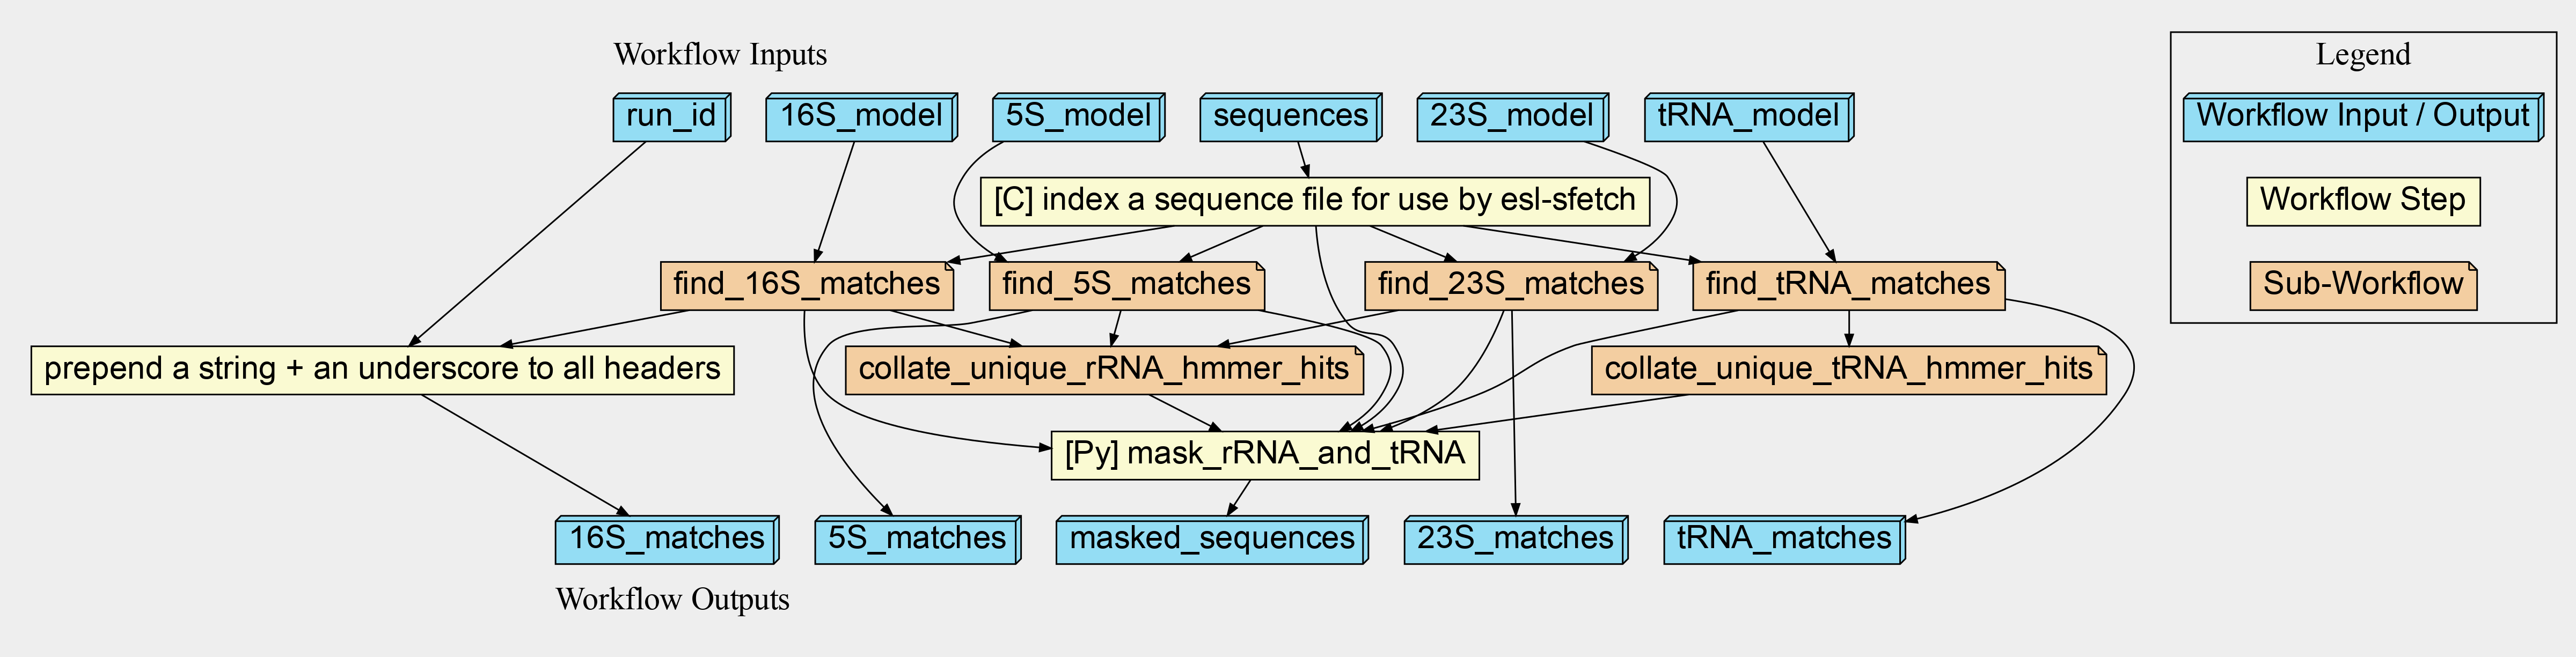
\includegraphics[width=\textwidth]{figure1}
  \caption{Excerpt from a large microbiome bioinformatics CWL workflow~\cite{mitchell_mgnify_2020}; this part of the workflow has the aim to match the Workflow Inputs of genomic sequences to provided sequence-models dispatched to four Sub-Workflows of further steps (not detailed above), outputs of which are then collated to identify unique sequence hits and provided as overall Workflow Outputs. Arrows define the dataflow between tasks, implying their partial ordering, shown here in layers of tasks that may execute concurrently.  Workflow Steps execute command line tools, shown here with indicators for their different programming languages: [Py] for Python; [C] for the C language. (Adapted from \url{https://w3id.org/cwl/view/git/7bb76f33bf40b5cd2604001cac46f967a209c47f/workflows/rna-selector.cwl} )}
  \label{fig:sample_workflow}
  \Description{TODO}
 \end{figure*}
 
In practice, many research and engineering groups use workflows of the kind described in Figure~\ref{fig:sample_workflow}. However, as highlighted in a recently published "Technology Toolbox" article~\cite{perkel_workflow_2019} published in the journal Nature, these groups lack the ability to share and collaborate across institutions and infrastructures without costly manual translation.

Currently many competing workflow management systems and runners exist, each with their own syntax or method for describing workflows and infrastructure requirements, which limit computational reuse and portability. The dataflows are becoming so complex, that their non-explicit specification in most workflow abstractions further increases the costs to reuse and port the workflow by third-parties.

We thus identify an important problem for the broad adoption of workflow thinking in practice: although communities want polylingual, and multi-party workflows, \textbf{adopting and managing different workflow systems is costly and difficult}. In this work, we propose to tame this complexity through a common abstraction that covers the majority of features used in practice, and is (or can be) implemented in many workflow systems.

In the computational workflow depicted in Figure~\ref{fig:sample_workflow}, practitioners solved their problem by adopting the \textbf{Common Workflow Language} (CWL), an open standard for describing command-line-tool based workflows like theirs. We posit in this work that CWL can help solve the main problems of sharing workflows between institutions and users, and we set out to introduce the CWL standards. CWL focuses on maintaining a separation of concerns between the description and execution of tools and workflows. CWL supports workflow automation, scalability, abstraction, provenance, portability, and reusability. Last, but not least, CWL takes a principled, community-first open-source and open-standard approach whcih enables this result.

CWL is the product of an open and free standards-making community. CWL began in the bioinformatics domain, but its principles are broad. Since the ratification of the first version in 2016, the CWL standards have seen use in other fields including hydrology\footnote{\url{https://www.eosc-portal.eu/eoscpilot-science-demonstrator-ewatercycle-switch-fair-data-hydrology}}, radio astronomy\footnote{\url{https://www.eosc-portal.eu/lofar-and-radio-astronomy-community}}, geo-spatial analysis~\cite{simonis_ogc_2020,goncalves_ogc_2020,landry_ogc_2020}, high energy physics~\cite{bell_web-based_2017} in addition to the more traditional bioinformatics fields like genomics and cancer research~\cite{kaushik_building_2019}. The many CWL contributors shaped the standard so that it could be useful to any domain that experiences the problem of "many tools written in many programming languages by many parties".

CWL could also be useful in computational domains beyond science. The separation of concerns CWL proposes enables diverse projects, and would also benefit engineering and large industrial projects. Likewise, users of software container technology like Docker that distribute analysis tools can use CWL for providing a structured workflow-independent description of how to run their tools, what data is required, and what results to expect.

HIGHLIGHTS BOX

Toward computational reuse and portability of polylingual, and multi-party workflows, CWL makes the following contributions:

\begin{enumerate}
\item
  {CWL is a set of standards for describing and sharing computational workflows,}
\item
  {CWL is used daily in many science and engineering domains, as well as by multi-stakeholder teams,}
\item
  {CWL has a \textit{declarative syntax}, facilitating polylingual workflow tasks. By being explicit about the \textit{runtime environment} and use of \textit{software containers}, CWL enables \textit{portability} and reuse,}
\item
  {The CWL standards provide a\textit{ separation of concerns} between workflow authors and workflow platforms,}
\item
  {The CWL standards support critical workflow concepts like automation, scalability, abstraction, provenance, portability, and reusability.}
\item
  {CWL is developed around core principles of community and shared decision making, re-use, and zero cost for participants.  (see section 4: Open Standards)}
\item
  {CWL is provided as freely-available open standards, supported by a diverse community in collaboration with industry, and a Free/Open Source Software ecosystem.}
\end{enumerate}

\section{Why Workflows?}

A process, digital or otherwise, may grow to such complexity that the authors and users of that process have difficulties in understanding its structure, scaling the process, managing the running of the process, and keeping track of what happened in previous enactments of the process. Process dependencies may be undocumented, obfuscated, or otherwise effectively invisible; even an extensively documented process may be difficult to understand by outsiders or newcomers if a common framework or vocabulary is lacking. A need to run the process more frequently or with larger inputs unrealistic to achieve by the sole entity (script or person) that was running the process initially. What was once a reasonable manual step (run this command here and then paste the result there; call this person for permission) may later be a bottleneck. Informal logs (if any) can quickly can become unsuitable for answering an organization's need to understand \textit{what} happened \textit{when} by \textit{whom} to \textit{which} data.

Workflow techniques aim to solve these problems by providing the "A.S.A.P." features : Abstraction, Scaling, Automation, and Provenance~\cite{cuevas-vicenttin_scientific_2012}.  Workflow constructs enable a clear abstraction about the \textit{components}, the \textit{relationships} between components, and the \textit{inputs} and \textit{outputs} of the components turning them into well-labeled tools with documented expectations. This abstraction enables \textit{scaling} (execution can be parallelized and distributed), \textit{automation} (the abstraction can be used by a workflow engine to track, plan, and manage execution of tasks), and \textit{provenance} tracking (descriptions of tasks, executors, inputs, outputs; with timestamps, identifiers, and other logs, can be stored in relation to each other to later answer structured queries).

Using workflow techniques, especially with digital analysis processes, has become quite popular and does not look to be slowing down: one platform recently celebrated its 10,000th citation \footnote{\url{https://galaxyproject.org/blog/2020-08-10k-pubs/}}; and over 285 computational workflow systems are known \footnote{\url{https://s.apache.org/existing-workflow-systems}}. However, except for systems adopting the CWL standards, every workflow system is incompatible with each other, each requiring users to express their computational workflows in a different way.

Local success, global \textit{un}portability. The success of workflows is now its biggest drawback: users are locked into a particular vendor, project, and often a particular hardware setup; thus sharing and re-use is hampered. Even non-academics suffer here, as the lack of standards (or the lack of their adoption) hinders effective collaboration on computational methods within and between companies. Likewise this \textit{unportability} affects public-private partnerships and potential for technology transfer from public researchers.

Sharing standards-based workflow descriptions may also help to solve a significant problem~\cite{ivie_reproducibility_2018, feitelson_repeatability_2015}: incomplete methods descriptions when computational analysis is reported in academic research. Reproduction, replication, or re-use of these digital methods requires a complete description of what computer applications were used, how exactly they were used, and how they were connected to each other. For precision and interoperability, this description should also be in an appropriate standardized machine-readable format.

\subsection{Sidebar A: Monolingual and Polylingual workflow systems}

Workflows techniques can be implemented in many ways with varying degrees of formalism which tends to correlate with execution flexibility and features. Typically the most informal techniques require that all processing components are written in the same programming language or are at least callable from the same programming language, while formal workflow techniques tend to allow components in multiple programming languages. 

On the informal side is the do-it-yourself approach using techniques built-in to a particular programming language: for example using the `threading' library in Python or MapReduce in Java using Apache Hadoop\cite{taylor_overview_2010}. To gain more flexibility (while still being based in a particular programming language) one might adopt a third-party library that can enable remote or distributed execution without having to re-write one's code like `ipyparallel' \footnote{\url{https://pypi.org/project/ipyparallel/}}.

A more explicit workflow structure can be achieved by using a programming language specific workflow library, like Parsl~\cite{babuji_parsl_2019}, where the workflow constructs("this is a unit of processing", "here are the dependencies between the units") are even more explicit, added to a Python script to upgrade it to a scaleble workflow. Here we list Parsl as an example of a \textbf{monolingual} workflow system, although it also contains explicit support for executing external command-line tools.

Two approaches are seen to accommodate workflows where the components are written in more than one programming language (or the components come from third parties and the user does not want to or cannot modify them): use of per-language \textit{add-in libraries} or the use of the \textbf{\textit{POSIX command-line interface}}~\cite{the_austin_group_posix1-2008_2008}. The use of per-language add-in libraries is done by either explicit function calls (e.g. using ctypes in Python to call a C library\footnote{\url{https://docs.python.org/3/library/ctypes.html}}) or the addition of annotations to the user's functions and requires mapping/restricting to a common cross-language data model.

Essentially all programming languages support the creation of \textit{POSIX}
command line interfaces familiar to many Linux and macOS users; scripts or binaries which can be invoked on the shell with a set of arguments, reading and writing files and executed in a separate process. Choosing the POSIX command-line interface as the point of coordination means the connection between components is done by an array of string \textit{arguments} representing program options (including paths to data files) along with a string-based \textit{environment variables} (KEY=value). This command-line option has the advantage of not needing per-language implementation at the expense of a very simple data model (and process start-up costs) which in workflows leads to a tendency for larger granularity of the units of work. As a \textit{\textbf{polylingual}} workflow standard, CWL uses the POSIX CLI data model.

\section{Features of the Common Workflow Language standards}

\begin{figure*}
  \centering
  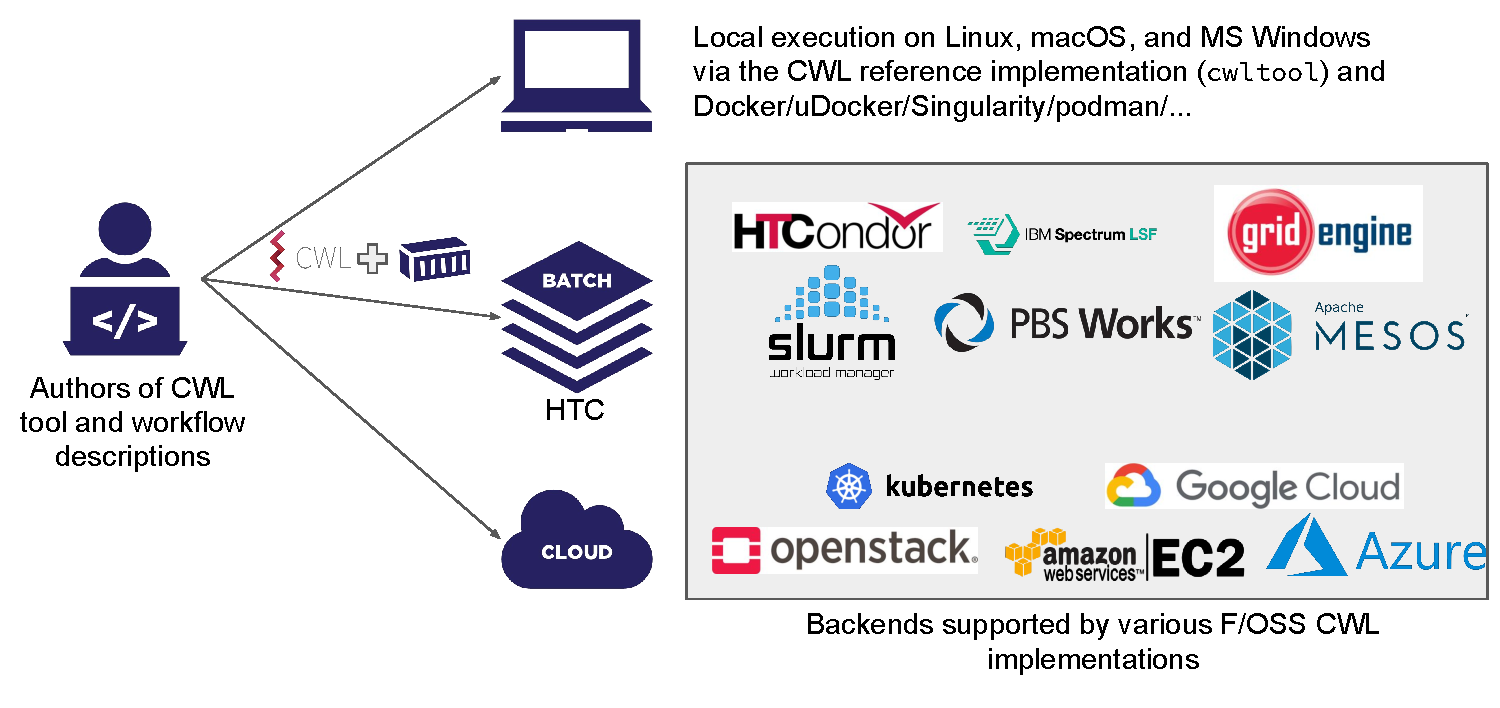
\includegraphics[width=\textwidth]{figure2}
  \caption{Example of CWL portability. The same workflow description runs on the scientist's own laptop or single machine, any batch production-environment, and any common public or private cloud. The CWL standards enable execution portability by being explicit about data locations. This enables execution of CWL workflows on diverse environments as provided by various implementations of the CWL standards: the scientist's own laptop or single machine, any batch production-environment, and any common public or private cloud.}
  \label{fig:portability}
  \Description{TODO}
\end{figure*}

Each release of CWL has two\footnote{There is a third component, the corresponding schema language standard \textit{Schema Salad} that is used to define the syntax of CWL itself.} main components (1) a standard for describing \textit{command line} tools; (2) a standard for describing \textit{workflows} that compose such tool descriptions. The goal of the \textbf{CWL Command Line Tool Description Standard}\footnote{\url{https://www.commonwl.org/v1.2/CommandLineTool.html}} is to describe how a particular command line tool works: what are the \textit{inputs} and \textit{parameters} and their types; how to add the correct flags and switches to the \textit{command line} invocation; and where to find the \textit{output files}. As shown in Figure 3B, item 3, these tool descriptions can contain \textit{hints} such as which software container to use or how much compute resources are required (memory, number of CPU cores, disk space, and/or
the maximum time.

\begin{figure*}
  \centering
  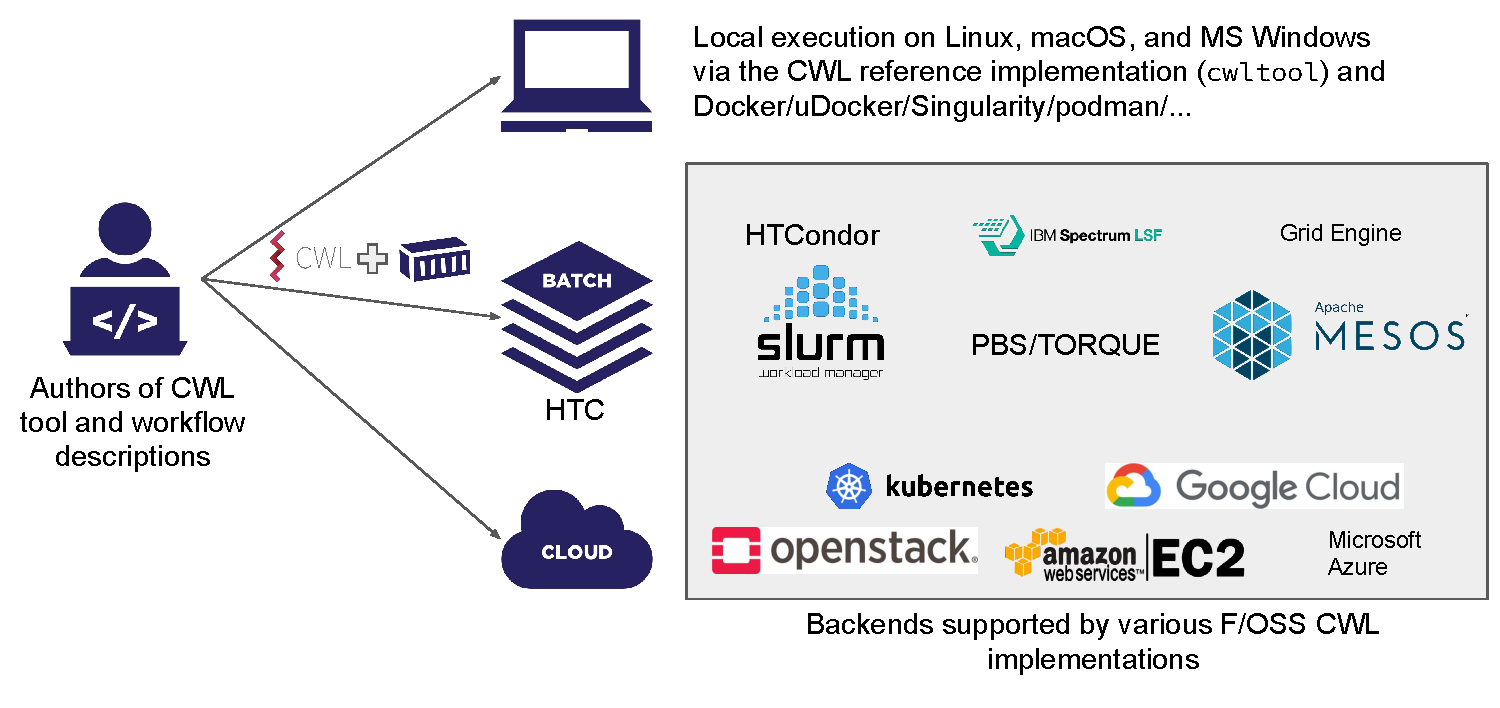
\includegraphics[width=\textwidth]{figure3}
  \caption{Example of CWL syntax and progressive enhancement. (A) and (B) describe the same tool, but (B) is enhanced with additional features: human-readable documentation, \textit{file format} identifiers validation of workflow connections; recommended \textit{software container} image for more reproducible results and easier software installation; dynamically specified \textit{resource requirements} to optimize task scheduling and resource usage without manual intervention.}
  \Description{TODO}
  \label{fig:syntax}
 \end{figure*}

CWL is a very explicit language, both in syntax and in its data and execution model. Textually one would write CWL in YAML\footnote{JSON is an acceptable subset of YAML, and common when converting from another format to CWL}, see Figure~\ref{fig:syntax}A for a simple example, and Figure~\ref{fig:syntax}B for the same execution augmented with further details. Each \textit{input} to a tool has a name and a type (e.g. File); likewise for the expected outputs. Tool description authors are encouraged to include \textit{documentation} and \textit{labels} for all components (Figure~\ref{fig:syntax}B), this enables automatic generation of helpful Graphical User Interfaces (GUIs) for any given CWL description. \textit{Metadata} about the tool description authors themselves encourages attribution of their efforts.

In the CWL execution model a tool's runtime environment is explicit and is controlled by the CWL tool description author \footnote{\url{https://www.commonwl.org/v1.2/CommandLineTool.html\#Runtime_environment}}. Each tool invocation uses a separate working directory, populated according to the CWL Tool description, e.g. explicit input files. For executing more "opinionated" applications, additional CWL constructs allow further customization of its runtime environment, e.g. particular file layout, additional static files or environment variables.

\textbf{Explicit runtime model enables portability} (as shown in Figure~\ref{fig:portability}) by being explicit about data locations. This enables execution of CWL workflows on diverse environments as provided by various implementations of the CWL standards: the local environment of the author-scientist (e.g., a single desktop computer, laptop, or workstation), a remote batch production-environment, and an on-demand cloud environment.

Using \textit{software container} technologies like Docker, which enables portability of the underlying analysis tools, is quite straightforward with CWL (Figure~\ref{fig:syntax}B, item 2): the workflow engine will handle mounting files and folders within the container. Indeed, the use of containers can be seen as a confirmation that a tool’s execution is reproducible using only its explicitly declared runtime environment. Likewise, no changes to a CWL tool description are needed when distributed execution is desired. As required file or directory inputs are always explicitly defined in the CWL description; the user's workflow platform can handle placement of jobs and routing of data between compute nodes without additional configuration.

The \textit{Common} Workflow Language standards aim to cover the common needs of users and the common\textit{ly} implemented features of workflow runners or platforms. To support features that are \textit{not} in the CWL standards there are well defined \textit{extension points} that permit namespaced vendor-specific features in well defined ways. If these extensions do not fundamentally change how the tool should operate then they are marked as "\textit{hints}" and other CWL engines can ignore them. However, if the extension is required to properly run the tool being described, perhaps due to the need for some exotic custom hardware, then the extension is listed under "\textit{requirements}" and other CWL engines can recognize their inability to execute that CWL description.

The \textbf{CWL Workflow Description Standard}\footnote{\url{https://www.commonwl.org/v1.2/Workflow.html}} builds upon the CWL Command Line Tool Standard: it has the same YAML/JSON style syntax with explicit workflow level inputs, outputs, and documentation. Here the workflow is formed by a list of \textit{steps} (made up of CWL CommandLineTools or CWL sub-Workflows), each re-exposing their tool's require \textit{inputs}, which are connected from either the common \textit{workflow inputs} or from step outputs of preceding steps; forming an explicit data-flow as required for the particular computational analysis. The \textit{workflow outputs} expose selected outputs from workflow steps (making explicit which intermediate step outputs will be returned from the workflow). All connections are made by identifiers, which CWL document authors are encouraged to make meaningful names for: "reference\_genome" instead of "input7". See Figure~\ref{fig:syntax} for an example.

This approach of modeling a workflow is the \textit{data flow paradigm}; the connectivity defines the partial execution order. Parallel execution of steps is permitted and encouraged whenever multiple steps have all of their inputs satisfied, or instance in Figure~\ref{fig:sample_workflow} \textit{find\_16S\_matches} and \textit{find\_S5\_matches} are at the same data dependency level and can execute concurrently or sequentially in any order. Additionally a "scatter" construct allows the repeated execution of a CWL step to \textit{iterate} or select from input arrays or multiples links to the same input. Starting with CWL version 1.2, workflows can also conditionally \textit{skip execution} of a (tool or workflow) step, based upon a specified intermediate input or custom boolean evaluation. Combining these features allows for a flexible branch mechanism while retaining the predictable data flow paradigm, which affords workflow engines to calculate data dependencies before the workflow starts.

The use of explicit runtime environments, combined with explicit inputs/outputs to form the data flow, means CWL workflows are more rigid to file layout changes and more flexible for step reordering and scalability compared to perhaps fragile approaches that rely on implicit file paths particular for the workflow, perhaps directly hard-coded in a tool or its arguments. In CWL individual tool definitions can be reused from multiple workflows, directly handle iterations and support scalable remote execution.

Forward compatibility of CWL documents is guaranteed as each CWL document declares which version of the standards it was written for. A stand alone upgrader\footnote{\url{https://pypi.org/project/cwl-upgrader/}} can automatically upgrade CWL documents from one version to the next, and many CWL-aware platforms will internally update user-submitted documents at runtime.

\section{Open-Source, Open Standards, Open Community}

Given the numerous and diverse set of potential users, implementers, and other stakeholders, we posit that a project like CWL requires combined development of code, standards, and community. Indeed, these requirements were part of the foundational design principles for CWL:

\textbf{Principle 1}: The core of the project is the community of people who cared about the goals.

\textbf{Principle 2}: To achieve the best possible results, there should be few, if any, barriers to participation in order to attract people with diverse experiences and perspectives; specifically there must be no cost to participate.

\textbf{Principle 3}: The outputs of this project should be as useful as possible to people in whatever way they can come up with, to enable the most good. Thus, the standards themselves must have no acquisition price and be licensed for reuse.

\textbf{Principle 4}: The project must not favor one company or group over another, but neither should it try to be all things to all people.

\textbf{Principle 5}: The concepts and ideas must be tested frequently, tested and functional code is the beginning of evaluating a proposal, not the end.

In time, the CWL project learned that this approach was a superset of the OpenStand Principles \footnote{https://open-stand.org/about-us/principles/} , a joint ``Modern Paradigm for Standards'' promoted by the IAB, IEEE, IETF, Internet Society, and W3C. The CWL addition to the OpenStand Principles is to keep participation free of cost, and the explicit choice of the Apache 2.0 license for all text, conformance tests, and the reference implementation.

\textbf{Necessary and sufficient}: All the principles have proven to be essential for the CWL project. For example, the free cost and open source license (Principle 2 and 3) has enabled many implementations of the CWL standards, several of which re-use different parts of the CWL reference runner. Being community-first (Principle 1) has led to several projects from participants that are outside the CWL standards themselves.

As part of Principle 5, we developed a suite of conformance tests for each version of the CWL standards. These publicly available tests were critical to CWL's success: they helped prove the reference implementation of CWL itself; they provided concrete examples to early adopters; and they enabled the developers and users of production implementations of the CWL standards to confirm their correctness.

\subsection{Sidebar C: CWL F/OSS Ecosystem}

\subsubsection{Free and Open Source implementations of CWL}\footnote{Snapshot of \url{https://www.commonwl.org/\#Implementations}}

Currently the CWL community does neither test nor certify CWL implementations, nor specific technology stacks. Platform/service providers can confirm support for a particular technology configuration and CWL. We recommend testing your desired technology stack using the CWL conformance tests. In addition to the implementations in Table \ref{tab:runners}, Galaxy~\cite{afgan_galaxy_2018}\footnote{\url{https://github.com/common-workflow-language/galaxy/pull/47}} and Pegasus~\cite{deelman_pegasus_2015}\footnote{\url{https://pegasus.isi.edu/documentation/manpages/pegasus-cwl-converter.html}} have in-development support for CWL as well.

\begin{table}
  \caption{Selected F/OSS workflow runners / platforms that implement the CWL standards}
  \label{tab:runners}
    \begin{tabular}{ll}
      \toprule
      Name & Platform support\\
      \midrule
      \href{https://pypi.org/project/cwltool}{cwltool} & Linux, macOS, Windows (via WSL 2) \\
      & local execution only\\
      \href{https://arvados.org}{Arvados} & in the cloud on AWS, Azure and GCP, \\
      & on premise \& hybrid clusters using Slurm\\
      \href{https://pypi.org/project/toil-cwl-runner}{Toil} & AWS, Azure, GCP, Grid Engine, HTCondor, \\
      & LSF, Mesos, OpenStack, Slurm, PBS/Torque\\
      & also local execution on Linux, macOS, \\
      & MS Windows (via WSL 2)\\
      \href{https://pypi.org/project/cwl-airflow}{CWL-Airflow} & Local execution on Linux, OS X\\
      & or via dedicated Airflow enabled cluster.\\
      \href{https://docs.reana.io/}{REANA} & Kubernetes, \href{https://clouddocs.web.cern.ch/clouddocs/containers/}{CERN OpenStack},\\
      & \href{https://wiki.openstack.org/wiki/Magnum}{OpenStack Magnum}\\
      \bottomrule
\end{tabular}
\end{table}

\subsubsection{F/OSS tools and libraries for CWL}\footnote{Summarized from \url{https://www.commonwl.org/\#Software_for_working_with_CWL}}

CWL plugins for text/code editors exist for Atom, vim, emacs, Visual Studio Code, IntelliJ, gedit, and any text editor that support the "language server" standard.

There are tools to generate CWL from Python (via argparse/click), Python (via functions), ACD, CTD, annotations in IPython Jupyter Notebooks. Libraries to generate and/or read CWL exist in many languages: Python, Java, R, Go, Scala, and C++.

\subsection{The CWL Ecosystem}

Beyond the ratified CWL standards that have been released over the last six years, the CWL community has made many tools, software libraries, connected specifications, and shared CWL descriptions for popular tools. For example, there are software development kits for both Python\footnote{\url{https://pypi.org/project/cwl-utils/}} and Java\footnote{\url{https://github.com/common-workflow-lab/cwljava}} that are generated automatically from the CWL schema; this allows programmers to load, modify, and save CWL documents using an object oriented model that has direct correspondence to the CWL standards themselves. CWL SDKs for other languages are possible by extending the code generation routines\footnote{See the “*codegen*.py” files in \url{https://github.com/common-workflow-language/schema_salad/tree/3cf7fafbdd07ecb448c32c939aca860173e598cf/schema_salad}}.

In response to the requests of many vendors for guidance on how to share workflow execution and authoring provenance information, the CWLProv\footnote{\url{https://w3id.org/cwl/prov/}} prototype was created to show how existing standards~\cite{belhajjame_using_2015,kunze_bagit_2018,missier_w3c_2013} can be combined to represent the provenance of a specific execution of a CWL workflow. At this time, CWLProv has only been implemented in the CWL reference runner, but interest is high in additional implementation and further development.

One criteria for evaluating a workflow language is the extent to which it supports a "separation of concerns" between the workflow description authors and the software implementers of the language. This separation of concerns is realized in CWL by using an explicit description approach. This has enabled several optimizations in scheduling (location-based~\cite{jiang_tr-19-01_2019}, cost-based\cite{jiang_pivot_2019}) and data-organization by researchers and other implementers of the CWL standards.

\section{Conclusion}

The problem of standardizing computational reuse is only increasing in prominence and impact. Various domains in science, engineering, and commerce have already started to migrate to workflows, but efforts focusing on the portability and even definition of workflows remain scattered. In this work we raise awareness to this problem and propose a community-driven solution.

The Common Workflow Language (CWL) is a family of standards for the description of command line tools and workflows made from these tools. It features support for software containers, resource requirements, and workflow-level conditional branching. Built on a foundation of five guiding principles, the CWL project delivers open standards, open source code, and an open community.

For the past six years, the community around CWL has developed organically, with plugins and converters for many systems, along with several production-grade implementations of the standards themselves.

To conclude: this is a call for others to embrace workflow thinking and join the CWL community!

\begin{acks}
The CWL project is immensely grateful to the following self-identified CWL Community members and their contributions to the project:
\href{https://orcid.org/0000-0002-2703-8936}{Miguel d'Arcangues Boland} (Software, Bug Reports, Maintenance),
Alain Domissy (Conceptualization, Answering Questions, Tools),
Andrey Kislyuk (Software, Bug Reports),
\href{https://orcid.org/0000-0001-7811-8613}{Brandi Davis-Dusenbery} (Conceptualization, Funding acquisition, Investigation, Project Administration, Resources, Supervision, Business
Development, Event Organizing, Talks),
\href{https://orcid.org/0000-0001-9795-7981}{Niels Drost} (Funding Acquisition, Blogposts, Event Organizing, Tutorials, Talks),
\href{https://orcid.org/0000-0001-8626-2148}{Robert Finn} (Data acquisition, Funding acquisition, Investigation, Resources, Supervision),
\href{https://orcid.org/0000-0001-9292-1533}{Michael Franklin} (Software, Bug Reports, Documentation, Event Organizing, Maintenance, Tools, Answering Questions, Talks),
\href{https://orcid.org/0000-0003-1550-1716}{Bogdan Gavrilovic} (Conceptualization, Software, Validation, Bug Reports, Blogposts, Maintenance, Tools, Answering Questions, Reviewed Contributions, User Testing),
\href{https://orcid.org/0000-0002-5843-4712}{Manabu Ishii} (Blogposts, Documentation, Examples, Event Organizing, Maintenance, Tools, Answering Questions, Translation, Tutorials, Talks),
\href{https://orcid.org/0000-0003-4115-3313}{Sinisa Ivkovic} (Software, Validation, Bug Reports, Tools),
\href{https://orcid.org/0000-0002-3468-0652}{Alexander Kanitz} (Software, Business Development, Tools, Talks),
\href{https://orcid.org/0000-0002-5044-4692}{Sehrish Kanwal} (Conceptualization, Formal Analysis, Investigation, Software, Validation, Bug Reports, Blogposts, Content, Event Organizing, Maintenance, Answering Questions, Tools, Tutorials, Talks, User Testing),
\href{https://orcid.org/0000-0001-9102-5681}{Andrey Kartashov} (Conceptualization, Software, Validation, Examples, Tools, Answering Questions),
\href{https://orcid.org/0000-0002-6337-3037}{Farah Khan} (Conceptualization, Formal Analysis, Funding Acquisition, Software),
\href{https://orcid.org/0000-0002-6486-3898}{Michael Kotliar} (Software, Validation, Bug Reports, Blogposts, Examples, Maintenance, Answering Questions, Reviewed Contributions, Tools, Talks, User Testing),
\href{https://orcid.org/0000-0003-1112-2284}{Folker Meyer} (Tools),
\href{https://orcid.org/0000-0002-6388-7353}{Rupert Nash} (Software, Bug Reports, Talks, Videos),
\href{https://orcid.org/0000-0003-3705-948X}{Maya Nedeljkovich} (Software, Validation, Visualization, Writing -\/- review \& editing, Bug Reports, Tools, Talks),
\href{https://orcid.org/0000-0003-3777-5945}{Tazro Ohta} (Formal Analysis, Funding Acquisition, Resources, Validation, Bug Reports, Blogposts, Content, Documentation, Examples, Event Organizing, Answering Questions, Tools, Translation, Tutorials, Talks, User Testing),
\href{https://orcid.org/0000-0002-8021-9162}{Pjotr Prins} (Blogposts, Packaging, Bug Reports),
\href{https://orcid.org/0000-0001-9279-9910}{Manvendra Singh} (Software, Blogposts, Packaging, Tools, Reviewed Contributions),
\href{https://orcid.org/0000-0002-0959-4429}{Andrey Tovchigrechko} (Conceptualization, Software, Bug Reports),
\href{https://orcid.org/0000-0003-3156-2105}{Alan Williams} (Investigation),
\href{https://orcid.org/0000-0002-6130-1021}{Denis Yuen} (Software, Bug Reports, Documentation, Tools),
\href{https://orcid.org/0000-0002-0415-9655}{Alexander (Sasha) Wait Zaranek} (Conceptualization, Funding Acquisition),
\href{https://orcid.org/0000-0003-4716-9121}{Sarah Wait Zaranek} (Conceptualization, Funding Acquisition, Project Administration, Resources, Software, Accessibility, Bug Reports, Business Development, Content, Examples, Event Organizing, Answering Questions, Tutorials, Talks).

The contributions to the CWL project by the authors of this paper are:
\href{https://orcid.org/0000-0002-2961-9670}{Michael R. Crusoe} (Conceptualization, Funding Acquisition, Investigation, Project Administration, Resources, Software, Supervision, Validation, Writing --- original draft, Bug Reports, Business Development, Content, Documentation, Examples, Event Organizing, Maintenance, Packaging, Answering Questions, Reviewing Contributions, Tutorials, Talks),
\href{https://orcid.org/0000-0002-2779-7174}{Sanne Abeln} (Writing --- original draft, and review \& editing, Conceptualization, Supervision, Funding acquisition)
\href{https://orcid.org/0000-0001-8030-9398}{Alexandru Iosup} (Writing --- original draft, and review, editing, Conceptualization, Supervision, Funding acquisition)
\href{https://orcid.org/0000-0003-3566-7705}{Peter Amstutz} (Conceptualization, Formal Analysis, Funding Acquisition, Methodology, Project Administration, Resources, Software, Supervision, Validation, Visualization, Bug Reports, Business Development, Content, Documentation, Examples, Event Organizing, Maintenance, Packaging, Answering Questions, Reviewed Contributions, Security, Tools, Tutorials, Talks),
\href{https://orcid.org/0000-0001-8316-4067}{Nebojša Tijanić} (Conceptualization, Software),
\href{https://orcid.org/0000-0002-7552-1009}{Hervé Ménager} (Conceptualization, Funding Acquisition, Investigation, Methodology, Project Administration, Resources, Software, Supervision, Bug Reports, Business Development, Examples, Event Organizing, Maintenance, Tools, Tutorials, Talks),
\href{https://orcid.org/0000-0001-9842-9718}{Stian Soiland-Reyes} (Conceptualization, Funding Acquisition, Investigation, Project Administration, Resources, Software, Supervision, Validation, User Testing, Bug Reports, Blogposts, Business Development, Content, Documentation, Examples, Event Organizing, Packaging, Tools, Answering Questions, Reviewed Contributions, Security, Tutorials, Talks, Videos),
\href{https://orcid.org/0000-0003-1219-2137}{Carole A. Goble} (Conceptualization, Funding Acquisition, Resources, Supervision, Audio, Business Development, Content, Examples, Event Organizing, Tools, Talks, Videos).

Funding acknowledgements: \grantsponsor{EU}{European Commission} via  \grantnum[https://cordis.europa.eu/project/id/823830]{EU}{H2020-INFRAEDI-02-2018 823830} BioExcel-2 (SSR), \grantnum[https://cordis.europa.eu/project/id/675728]{EU}{H2020-EINFRA-2015-1 675728} BioExcel (SSR), \grantnum[https://cordis.europa.eu/project/id/824087]{EU}{H2020-INFRAEOSC-2018-2 824087} EOSC-Life (SSR), \grantnum[https://cordis.europa.eu/project/id/739563]{EU}{H2020-INFRADEV-2016-2 739563} EOSCPilot (MRC), \grantnum[https://cordis.europa.eu/project/id/730976]{EU}{H2020-INFRAIA-2017-1-two-stage 730976} IBISBA 1.0 (SSR), \grantnum[https://cordis.europa.eu/project/id/676559]{EU}{H2020-INFRADEV-1-2015-1 676559} ELIXIR-EXCELERATE (SSR, HM).

\end{acks}

%%
%% The next two lines define the bibliography style to be used, and
%% the bibliography file.
\bibliographystyle{ACM-Reference-Format}
\bibliography{references}

%%
%% If your work has an appendix, this is the place to put it.
%% \appendix



\end{document}
\endinput